\documentclass{article}

\usepackage{../../../preamble}

\title{Deep Learning In Practice: Homework 5}
\author{Mahdi Kallel, Noureddine Sedki, Raphael Reme}

\begin{document}
\maketitle

\section{Introduction}

The goal of this assignment is to learn to predict correctly trajectories of Rössler systems. In such a system, each trajectory
$\left\{W_t = (x_t, y_t, z_t)^T\right\}_{t \ge 0}$ follows a simple temporal ODE:

\begin{equation*}
    \dot{W_t} = f(W_t) = \Bigg\{ \begin{aligned}
         & - y_t - z_t     \\
         & x_t + ay_t      \\
         & b + z_t(x_t -c) \\
    \end{aligned}
\end{equation*}

With $a, b, c$ some parameters. In this experiment, we will focus on the predefined value $a=0.2$, $b=0.2$, and $c=5.7$.

The trajectories of such system are deterministic but chaotic: A minor deviation leads to a very different trajectory. Our goal is to create a
model that is able to predict the trajectory given a starting point.


\begin{figure}[h!]
    \centering
    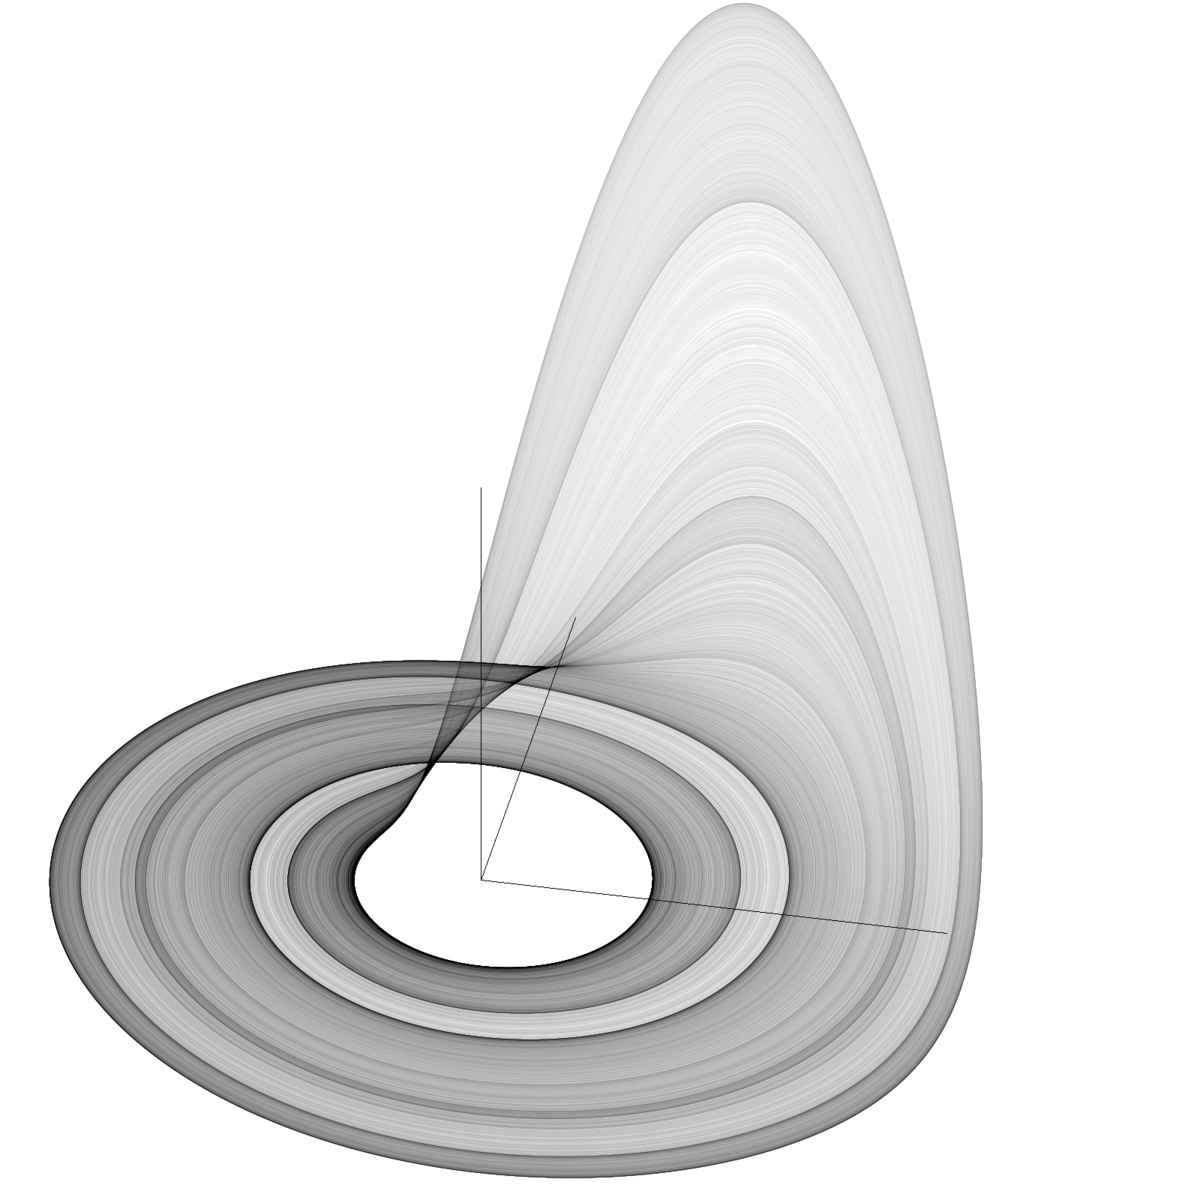
\includegraphics[width=0.5\linewidth]{rossler_attractor}
    \caption{One typical trajectory \\(https://en.wikipedia.org/wiki/Rossler\_attractor)}
    \label{fig:typical}
\end{figure}

\section{Chosen Approach}
We were proposed several approaches to solve this problem:
\begin{enumerate}
    \item Continuous system: Use a Neural Network to predict directly the derivative ($\dot{W_t} = \text{NN}(W_t)$).
    \item Discrete system without memory: Use a Neural Network to predict the next state ($W_{t + dt} = \text{NN}(W_t)$).
    \item Discrete system with memory: Use a Recurrent Neural Network to predict the next state ($W_{t + dt}, H_{t_+dt} = \text{RNN}(W_t, H_t)$).
\end{enumerate}

We have chosen to go with the second approach as it is straightforward to set it up. Indeed we do not need to compute the true $\dot{W_t}$ to regress it,
nor compute $W_{t + dt}$ from this regression as it would have been needed for the first approach. Moreover we can use directly the whole state
(no embedding) and the jacobian (that is needed later) is easy to compute, which is not the case for the third approach.

\subsection{Architecture}
With this approach, a simple architecture should be enough. We have decided to use a simple feed-forward architecture with only linear layers and
ReLU activation. We found that having at least a width of 100 helped the training to converge quickly, and we used only 4 layers to prevent exploding
gradient.

Finally the architecture that we used is a feed-forward network composed of 4 layers:
\begin{enumerate}
    \item Linear layer of size (3 x 50) + ReLU
    \item Linear layer of size (50 x 100) + ReLU
    \item Linear layer of size (100 x 200) + ReLU
    \item Linear layer of size (200 x 3)
\end{enumerate}

\subsection{Dataset}
In order to learn correctly the dynamics of the system we have to generate a dataset that represent well the problem. In this state of mind, for
the training dataset we have generated several trajectories from different initial points of duration 200s (Enough to perform several circles).
We have chosen the initial points either randomly inside the typical distribution of one long trajectory, or near the equilibrium point.
(Without it the space near the equilibrium point is unknown for network as no trajectory starting far from it will converge toward it.)

We have used a $\Delta_t$ of 0.1s as smaller ones (0.01 and 0.001) did not yield good trajectories. With this large $\Delta_t$ we are able to
handle longer trajectories.

At training time we have found that using a single trajectory in each batch was more efficient.

Finally we have also used a validation set with different initialization points (sampled as described above) and keep the best model
with respect to a Mean Square Error on this validation set between the predicted trajectory and the true trajectory.

\subsection{Loss}
We focus on a simple MSE loss. But we tried to improve training with more complexe predictions: Instead of only predicting the next sample we tried to
predict the N-next samples for each batch. The idea is to let the network learn the real autoregressive task on n-sample and not just focus on the next
one. Given $W_t$ we compute $\hat{W}_{t + i dt} = \text{NN}^{i}(W_t)$. And the loss is simply the MSE over each computed $\hat{W}_{t + i dt}$.

This approach is not stable for large value of N (As we stack the same network several times, we are facing exploding gradient issues). It
gives good results with $N \le 10$, nonetheless it didn't not really improve the results of $N=1$.

\section{Results analysis}
We would like to compute some quantities in order to be sure that our model is able to generate good trajectories. In the training we have only check
a MSE criterion. Here we will try to estimate the global quality of the trajectory with other features.

\subsection{PDF}
The idea here is to check that the distribution over each axis is the same for the predicted and true trajectory. The figure \ref{fig:pdf} shows clearly
that the predicted trajectory has the same distribution than the true one.

\begin{figure}[h!]
    \centering
    \begin{subfigure}[b]{0.3\linewidth}
        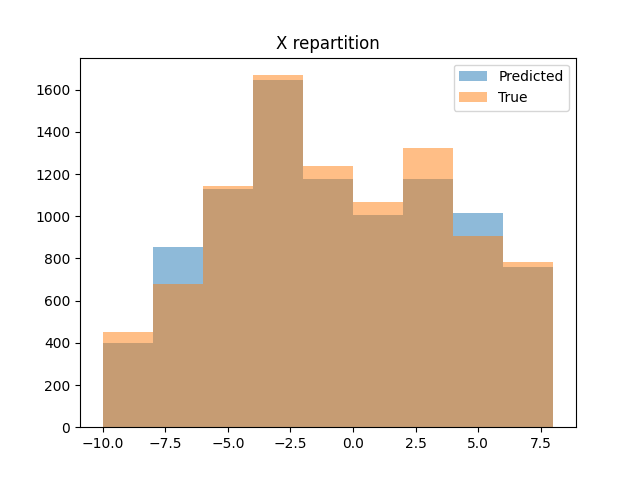
\includegraphics[width=\linewidth]{x_density}
    \end{subfigure}
    \begin{subfigure}[b]{0.3\linewidth}
        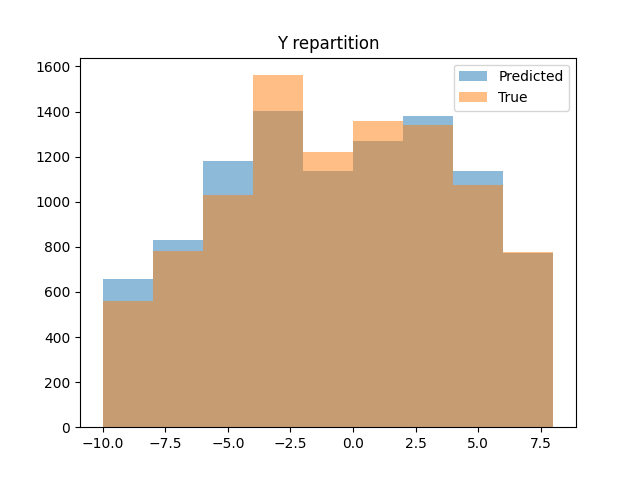
\includegraphics[width=\linewidth]{y_density}
    \end{subfigure}
    \begin{subfigure}[b]{0.3\linewidth}
        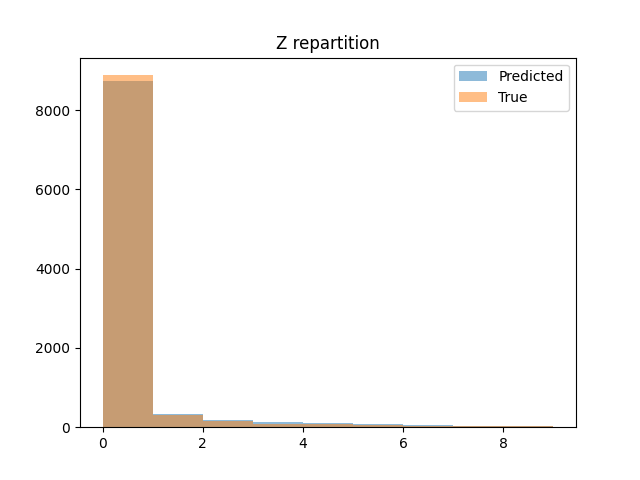
\includegraphics[width=\linewidth]{z_density}
    \end{subfigure}
    \caption{Distribution over each axis}
    \label{fig:pdf}
\end{figure}

\subsection{Time correlation}
We have computed the autocorrelation function for each trajectory (only with $y_t$ as it is a sufficient embedding for the whole trajectory).
As one can see they are very similar, which indicates that they have similar pseudo periods.

\begin{figure}[h!]
    \centering
    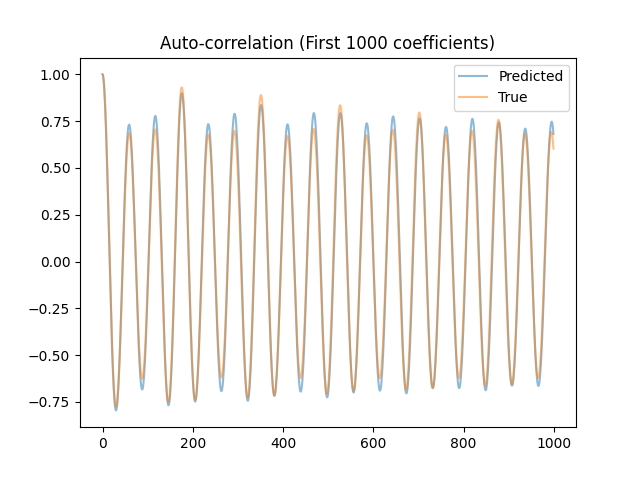
\includegraphics[width=0.4\linewidth]{auto-correlation}
    \caption{Autocorrelation function for lags betwen 0 and 100s}
    \label{fig:autocorrelation}
\end{figure}

\subsection{Fourier transform}
We have compared the main frequencies for each trajectory. They are also very similar which is not a suprise, as we already showed some
time correlation.

\begin{figure}[h!]
    \centering
    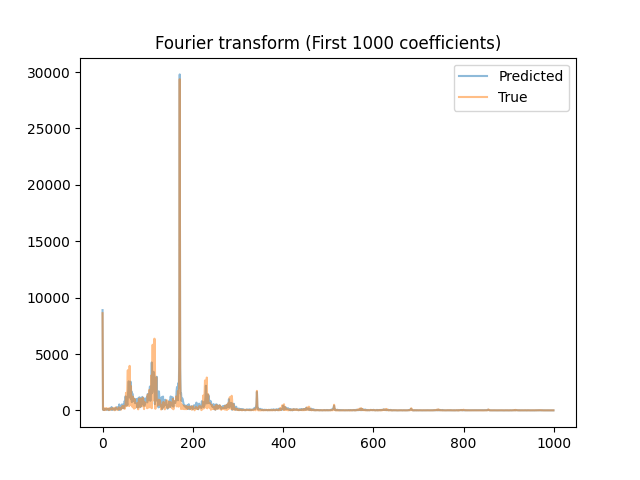
\includegraphics[width=0.4\linewidth]{fourier}
    \caption{Main fourier coefficients}
    \label{fig:fourier}
\end{figure}

\subsection{Equilibrium point}
We tried to find the equilibrium point of our network, and compare it with the real equilibrium point of the system. We have found that the equilibrium
point of our network $(0.009, -0.036, 0.034)$ is very close of the true equilibrium point $(0.007, -0.035, 0.035)$.\\
Nonetheless as there are very litle movements near the equilibrium point, our network has learnt a stable (or more stable) equilibrium.
Given a point near the equilibrium the trajectory will stay close to the equilibrium. (whereas the true trajectory diverts slowly).

\subsection{Lyapunov exponents}
We have finally computed the first Lyapunov exponent of the predicted trajectory that should be around $7e-2$ as for the true trajectory.

We have found a Lyapunov exponent of $6.4e-2$.

\section{Reproducing results}
In order to reproduce the training of the model, run the command:

\begin{lstlisting}{bash}
    $ python train.py
\end{lstlisting}
If you have a trained model, you can run
\begin{lstlisting}{bash}
    $ python TP.py
\end{lstlisting}
This command will output all the figures and analysis required.\\
These commands accept a list of options, but the default one are those that we finally used (use -h to see them)

\section{Conclusion}
We are able to generate quite good trajectories with a simple neural network that predicts the next point with a time delta of 0.1s. Even though errors
stack at each new prediction, the global quality of the trajectory is conserved but it struggles to fit the extreme points.

\begin{figure}[h!]
    \centering
    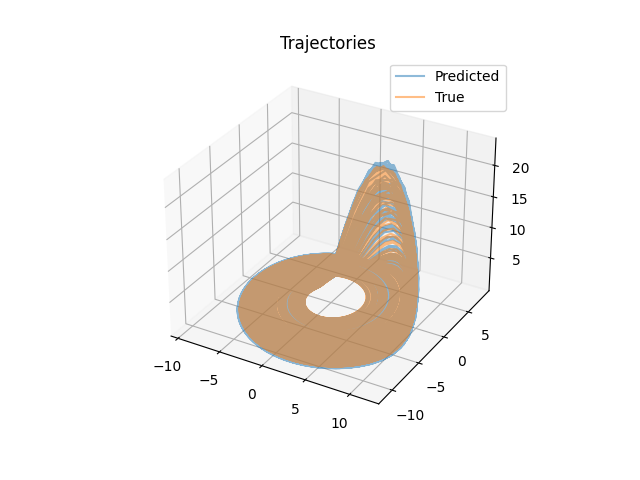
\includegraphics[width=0.4\linewidth]{trajectory}
    \caption{An example of 1000 seconds}
    \label{fig:example}
\end{figure}

\end{document}
